\documentclass[a4paper, 12pt]{article}
\usepackage[utf8]{inputenc} 
\usepackage{svg}
\usepackage{hyperref}
\usepackage{tikz}
\usepackage{mathtools}
\usepackage{wrapfig}
\usepackage{enumerate}
\usepackage{amsmath}
\usepackage{adjustbox}
\usepackage{graphicx}
\usepackage[T2A]{fontenc}
\usepackage[utf8]{inputenc}
\usepackage{booktabs,tabularx}
\usepackage{makecell}
\usepackage[most]{tcolorbox}
\usepackage{minted}
\usepackage[T2A]{fontenc} 
\usepackage[english,russian,ukrainian]{babel}


\definecolor{block-gray}{gray}{0.90} % уровень прозрачности (1 - максимум)
\graphicspath{{graphic/}}
\newtcolorbox{test-answer}{colback=block-gray,grow to right by=-10mm,grow to left by=-10mm,
boxrule=1pt,boxsep=0pt,breakable} % настройки области с изменённым фоном
\newtcolorbox{test-answer-long}{colback=block-gray,
boxrule=1pt,boxsep=0pt,breakable} % настройки области с изменённым фоном



\title{Завдання 6.02}
\author{Бездушний Вадим \textbf{K-24}}
\date{}



\begin{document}
\maketitle

\section{Відповіді на тест}
\begin{enumerate}
\item{B}
\item{B}
\item{C}
\item{D}
\item{D}
\item{B}
\item{C}
\item{A}
\item{A}
\item{A}
\end{enumerate}
\section{Опишіть можливості та реалізації технології ORM}
\textbf{ORM} \textit{(Object Relational Mapping)} --- технологія, що зв’язує реальну базу даних та концепції \textit{ООП}.
Основні можливості і переваги ORM:
\begin{itemize}
\item{Без ORM розробнику треба писати SQL код самостійно, більша вірогідність допустити помилки}
\item{Код, генеруємий ORM оптимізований, полегшується робота розробника}
\item{Розробник працює з об’єктами, віддаючи ORM обробку реляційних зв’язків}
\end{itemize}
В моїй лабараторній мене цікавить реалізація ORM для мови Python. Така система існує і називається \textbf{SQLAlchemy}. В SQLAlchemy впроваджено шаблон \textit{Data Mapper} (подібний на Hibernate для Java) замість шаблону \textit{active Record} який використовується в багатьох інших об'єктно-реляційних відображеннях.
\section{ER-діаграма}
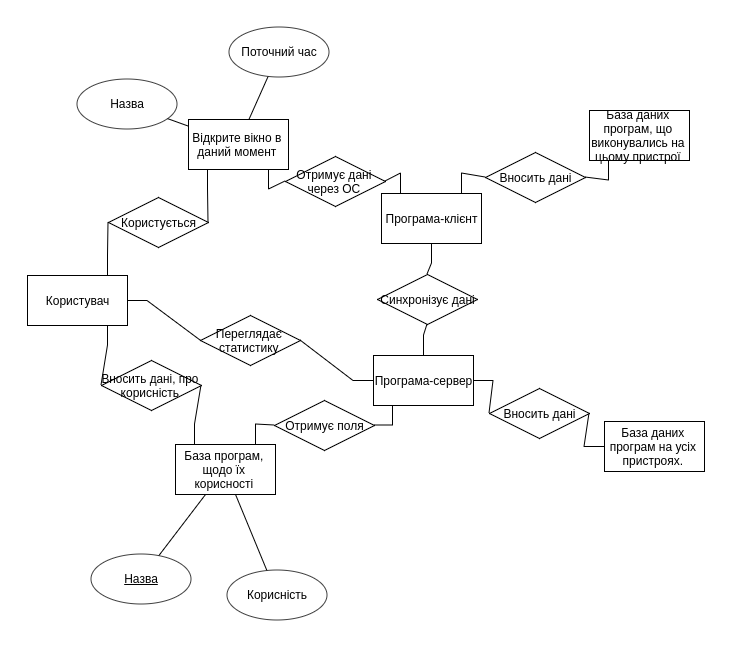
\includegraphics[width=\textwidth]{erdiagram.png}
\end{document}
